% $Id: notes.tex,v 1.94 2021/03/23 17:18:17 brandenb Exp $
%\documentclass{article}
\documentclass[twocolumn]{article}
\setlength{\textwidth}{160mm}
\setlength{\oddsidemargin}{-0mm}
\setlength{\textheight}{220mm}
\setlength{\topmargin}{-8mm}
\usepackage{graphicx,natbib,bm,url,color}
\graphicspath{{./fig/}{./png/}}
\thispagestyle{empty}
\input macros
\def\red{\textcolor{red}}
\def\blue{\textcolor{blue}}
\title{Measuring the correlation time}
\author{Axel Brandenburg}
\date{\today,~ $ $Revision: 1.94 $ $}
\begin{document}
\maketitle

%\section{}

%Use $(r,\phi,z)$ coordinates and

%\begin{itemize}\itemsep-0.2mm
%\item
%\end{itemize}

Compute
\begin{equation}
\tau_{\uu^2}(t)=\int_0^t \bra{\uu(t)\cdot\uu(t')}\,\dd t'/\bra{\uu^2}.
\end{equation}
\begin{equation}
\tau_{\oo\cdot\uu}(t)=\int_0^t \bra{\oo(t)\cdot\uu(t')}\,\dd t'/\bra{\oo\cdot\uu}.
\end{equation}
\begin{equation}
\tau_{\uu\cdot\oo}(t)=\int_0^t \bra{\uu(t)\cdot\oo(t')}\,\dd t'/\bra{\oo\cdot\uu}.
\end{equation}
\begin{equation}
\tau_{\uu\cdot\oo}(t)=\bbra{\uu(t)\cdot\int_0^t \oo(t')\,\dd t'}/\bra{\oo\cdot\uu}.
\end{equation}
see \Fig{pcortime} for a case where $\kf=10$ and $\urms=0.1$.
$\bra{\uu^2}$
\begin{equation}
\tau(t,k)=\int_0^t \Sp_k\left[\uu(t),\uu(t')\right]\,\dd t'/\bra{F(k)},
\end{equation}
where $\Sp(a,b)=a_k b_b^* + \mbox{c.c.}$ and $F(k)$ is the helicity spectrum.

\begin{figure}[h!]\begin{center}
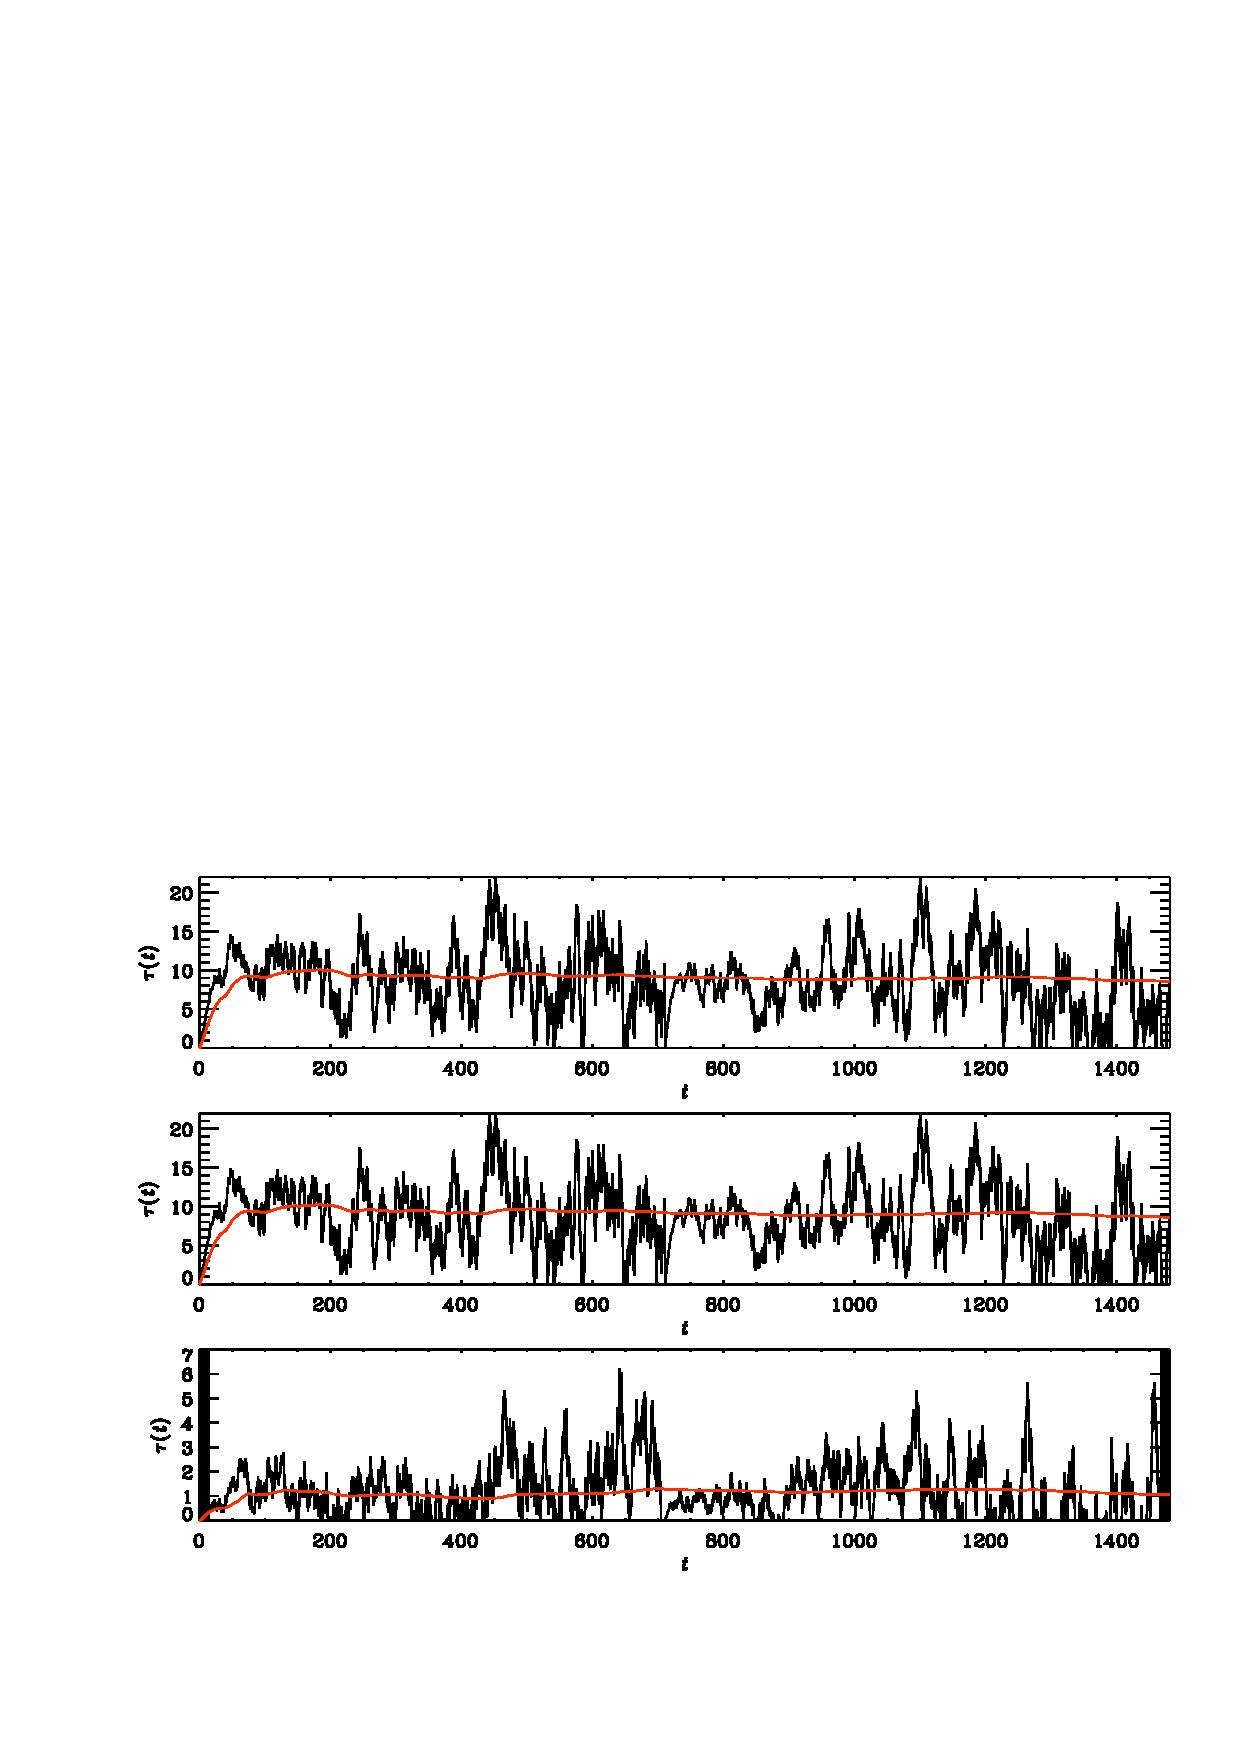
\includegraphics[width=\columnwidth]{pcortime}
\end{center}\caption[]{
\url{pcortime}
}\label{pcortime}\end{figure}

%\begin{table}[htb]\caption{
%}\vspace{12pt}\centerline{\begin{tabular}{lccccccc}
%$R$ & $T$ & $\kf$ & $\omf$ & $\EEGW$ & $\hrms$ & $k_{\rm peak}$ \\
%\hline
%\label{Ttimescale}\end{tabular}}\end{table}

%r e f
%\begin{thebibliography}{}

%\bibitem[Biskamp \& M\"uller(1999)]{BM99}
%Biskamp, D., \& M\"uller, W.-C.\yprl{1999}{83}{2195}

%\end{thebibliography}

%\vfill\bigskip\noindent\tiny\begin{verbatim}
%$Header: /var/cvs/brandenb/tex/etc/notes.tex,v 1.94 2021/03/23 17:18:17 brandenb Exp $
%\end{verbatim}

\end{document}
